% Options for packages loaded elsewhere
\PassOptionsToPackage{unicode}{hyperref}
\PassOptionsToPackage{hyphens}{url}
%
\documentclass[
]{article}
\usepackage{lmodern}
\usepackage{amssymb,amsmath}
\usepackage{ifxetex,ifluatex}
\ifnum 0\ifxetex 1\fi\ifluatex 1\fi=0 % if pdftex
  \usepackage[T1]{fontenc}
  \usepackage[utf8]{inputenc}
  \usepackage{textcomp} % provide euro and other symbols
\else % if luatex or xetex
  \usepackage{unicode-math}
  \defaultfontfeatures{Scale=MatchLowercase}
  \defaultfontfeatures[\rmfamily]{Ligatures=TeX,Scale=1}
\fi
% Use upquote if available, for straight quotes in verbatim environments
\IfFileExists{upquote.sty}{\usepackage{upquote}}{}
\IfFileExists{microtype.sty}{% use microtype if available
  \usepackage[]{microtype}
  \UseMicrotypeSet[protrusion]{basicmath} % disable protrusion for tt fonts
}{}
\makeatletter
\@ifundefined{KOMAClassName}{% if non-KOMA class
  \IfFileExists{parskip.sty}{%
    \usepackage{parskip}
  }{% else
    \setlength{\parindent}{0pt}
    \setlength{\parskip}{6pt plus 2pt minus 1pt}}
}{% if KOMA class
  \KOMAoptions{parskip=half}}
\makeatother
\usepackage{xcolor}
\IfFileExists{xurl.sty}{\usepackage{xurl}}{} % add URL line breaks if available
\IfFileExists{bookmark.sty}{\usepackage{bookmark}}{\usepackage{hyperref}}
\hypersetup{
  pdftitle={INLArethinking\_HW4},
  pdfauthor={Ania Kawiecki},
  hidelinks,
  pdfcreator={LaTeX via pandoc}}
\urlstyle{same} % disable monospaced font for URLs
\usepackage[margin=1in]{geometry}
\usepackage{color}
\usepackage{fancyvrb}
\newcommand{\VerbBar}{|}
\newcommand{\VERB}{\Verb[commandchars=\\\{\}]}
\DefineVerbatimEnvironment{Highlighting}{Verbatim}{commandchars=\\\{\}}
% Add ',fontsize=\small' for more characters per line
\usepackage{framed}
\definecolor{shadecolor}{RGB}{248,248,248}
\newenvironment{Shaded}{\begin{snugshade}}{\end{snugshade}}
\newcommand{\AlertTok}[1]{\textcolor[rgb]{0.94,0.16,0.16}{#1}}
\newcommand{\AnnotationTok}[1]{\textcolor[rgb]{0.56,0.35,0.01}{\textbf{\textit{#1}}}}
\newcommand{\AttributeTok}[1]{\textcolor[rgb]{0.77,0.63,0.00}{#1}}
\newcommand{\BaseNTok}[1]{\textcolor[rgb]{0.00,0.00,0.81}{#1}}
\newcommand{\BuiltInTok}[1]{#1}
\newcommand{\CharTok}[1]{\textcolor[rgb]{0.31,0.60,0.02}{#1}}
\newcommand{\CommentTok}[1]{\textcolor[rgb]{0.56,0.35,0.01}{\textit{#1}}}
\newcommand{\CommentVarTok}[1]{\textcolor[rgb]{0.56,0.35,0.01}{\textbf{\textit{#1}}}}
\newcommand{\ConstantTok}[1]{\textcolor[rgb]{0.00,0.00,0.00}{#1}}
\newcommand{\ControlFlowTok}[1]{\textcolor[rgb]{0.13,0.29,0.53}{\textbf{#1}}}
\newcommand{\DataTypeTok}[1]{\textcolor[rgb]{0.13,0.29,0.53}{#1}}
\newcommand{\DecValTok}[1]{\textcolor[rgb]{0.00,0.00,0.81}{#1}}
\newcommand{\DocumentationTok}[1]{\textcolor[rgb]{0.56,0.35,0.01}{\textbf{\textit{#1}}}}
\newcommand{\ErrorTok}[1]{\textcolor[rgb]{0.64,0.00,0.00}{\textbf{#1}}}
\newcommand{\ExtensionTok}[1]{#1}
\newcommand{\FloatTok}[1]{\textcolor[rgb]{0.00,0.00,0.81}{#1}}
\newcommand{\FunctionTok}[1]{\textcolor[rgb]{0.00,0.00,0.00}{#1}}
\newcommand{\ImportTok}[1]{#1}
\newcommand{\InformationTok}[1]{\textcolor[rgb]{0.56,0.35,0.01}{\textbf{\textit{#1}}}}
\newcommand{\KeywordTok}[1]{\textcolor[rgb]{0.13,0.29,0.53}{\textbf{#1}}}
\newcommand{\NormalTok}[1]{#1}
\newcommand{\OperatorTok}[1]{\textcolor[rgb]{0.81,0.36,0.00}{\textbf{#1}}}
\newcommand{\OtherTok}[1]{\textcolor[rgb]{0.56,0.35,0.01}{#1}}
\newcommand{\PreprocessorTok}[1]{\textcolor[rgb]{0.56,0.35,0.01}{\textit{#1}}}
\newcommand{\RegionMarkerTok}[1]{#1}
\newcommand{\SpecialCharTok}[1]{\textcolor[rgb]{0.00,0.00,0.00}{#1}}
\newcommand{\SpecialStringTok}[1]{\textcolor[rgb]{0.31,0.60,0.02}{#1}}
\newcommand{\StringTok}[1]{\textcolor[rgb]{0.31,0.60,0.02}{#1}}
\newcommand{\VariableTok}[1]{\textcolor[rgb]{0.00,0.00,0.00}{#1}}
\newcommand{\VerbatimStringTok}[1]{\textcolor[rgb]{0.31,0.60,0.02}{#1}}
\newcommand{\WarningTok}[1]{\textcolor[rgb]{0.56,0.35,0.01}{\textbf{\textit{#1}}}}
\usepackage{longtable,booktabs}
% Correct order of tables after \paragraph or \subparagraph
\usepackage{etoolbox}
\makeatletter
\patchcmd\longtable{\par}{\if@noskipsec\mbox{}\fi\par}{}{}
\makeatother
% Allow footnotes in longtable head/foot
\IfFileExists{footnotehyper.sty}{\usepackage{footnotehyper}}{\usepackage{footnote}}
\makesavenoteenv{longtable}
\usepackage{graphicx,grffile}
\makeatletter
\def\maxwidth{\ifdim\Gin@nat@width>\linewidth\linewidth\else\Gin@nat@width\fi}
\def\maxheight{\ifdim\Gin@nat@height>\textheight\textheight\else\Gin@nat@height\fi}
\makeatother
% Scale images if necessary, so that they will not overflow the page
% margins by default, and it is still possible to overwrite the defaults
% using explicit options in \includegraphics[width, height, ...]{}
\setkeys{Gin}{width=\maxwidth,height=\maxheight,keepaspectratio}
% Set default figure placement to htbp
\makeatletter
\def\fps@figure{htbp}
\makeatother
\setlength{\emergencystretch}{3em} % prevent overfull lines
\providecommand{\tightlist}{%
  \setlength{\itemsep}{0pt}\setlength{\parskip}{0pt}}
\setcounter{secnumdepth}{-\maxdimen} % remove section numbering

\title{INLArethinking\_HW4}
\author{Ania Kawiecki}
\date{8/3/2020}

\begin{document}
\maketitle

\href{https://github.com/rmcelreath/statrethinking_winter2019/tree/master/homework}{Statistical
rethinking homework solutions}

\href{https://becarioprecario.bitbucket.io/inla-gitbook/ch-intro.html}{INLA
book}

\begin{Shaded}
\begin{Highlighting}[]
\KeywordTok{library}\NormalTok{(tidyverse)}
\KeywordTok{library}\NormalTok{(rethinking)}
\KeywordTok{library}\NormalTok{(dagitty)}
\KeywordTok{library}\NormalTok{(INLA)}
\KeywordTok{library}\NormalTok{(knitr)}
\end{Highlighting}
\end{Shaded}

\hypertarget{homework-4}{%
\section{HOMEWORK 4}\label{homework-4}}

\hypertarget{section}{%
\subsection{1.}\label{section}}

Consider three fictional Polynesian islands. On each there is a Royal
Ornithologist charged by the king with surveying the bird population.
They have each found the following proportions of 5 important birb
species:

\begin{Shaded}
\begin{Highlighting}[]
\NormalTok{IB1 <-}\StringTok{ }\KeywordTok{c}\NormalTok{( }\FloatTok{0.2}\NormalTok{ , }\FloatTok{0.2}\NormalTok{ , }\FloatTok{0.2}\NormalTok{ , }\FloatTok{0.2}\NormalTok{ , }\FloatTok{0.2}\NormalTok{ )}
\NormalTok{IB2<-}\StringTok{ }\KeywordTok{c}\NormalTok{( }\FloatTok{0.8}\NormalTok{ , }\FloatTok{0.1}\NormalTok{ , }\FloatTok{0.05}\NormalTok{ , }\FloatTok{0.025}\NormalTok{ , }\FloatTok{0.025}\NormalTok{ )}
\NormalTok{IB3 <-}\StringTok{ }\KeywordTok{c}\NormalTok{( }\FloatTok{0.05}\NormalTok{ , }\FloatTok{0.15}\NormalTok{ , }\FloatTok{0.7}\NormalTok{ , }\FloatTok{0.05}\NormalTok{ , }\FloatTok{0.05}\NormalTok{ )}

\NormalTok{df <-}\StringTok{ }\KeywordTok{data.frame}\NormalTok{(IB1, IB2, IB3)}

\KeywordTok{rownames}\NormalTok{(df) <-}\StringTok{ }\KeywordTok{c}\NormalTok{(}\StringTok{"A"}\NormalTok{, }\StringTok{"B"}\NormalTok{, }\StringTok{"C"}\NormalTok{, }\StringTok{"D"}\NormalTok{, }\StringTok{"E"}\NormalTok{)}

\KeywordTok{kable}\NormalTok{(df)}
\end{Highlighting}
\end{Shaded}

\begin{longtable}[]{@{}lrrr@{}}
\toprule
& IB1 & IB2 & IB3\tabularnewline
\midrule
\endhead
A & 0.2 & 0.800 & 0.05\tabularnewline
B & 0.2 & 0.100 & 0.15\tabularnewline
C & 0.2 & 0.050 & 0.70\tabularnewline
D & 0.2 & 0.025 & 0.05\tabularnewline
E & 0.2 & 0.025 & 0.05\tabularnewline
\bottomrule
\end{longtable}

Notice that each column sums to 1, all the birbs. This problem has two
parts. It is not computationally complicated. But it is conceptually
tricky.

First, compute the entropy of each island's birb distribution. Interpret
these entropy values.

Second, use each island's birb distribution to predict the other two.
This means to compute the K-L Divergence of each island from the others,
treat- ing each island as if it were a statistical model of the other
islands. You should end up with 6 different K-L Divergence values. Which
island predicts the others best? Why?

SOL: To compute the entropies,we just need a function to compute the
entropy.Information entropy, as defined in lecture and the book, is
simply: \(H(p) = - \sum_{i}p_i log(p_i)\)

where p is a vector of probabilities summing to 1. In R code this would
look like:

\begin{Shaded}
\begin{Highlighting}[]
\NormalTok{H <-}\StringTok{ }\ControlFlowTok{function}\NormalTok{(p) }\OperatorTok{-}\KeywordTok{sum}\NormalTok{(p}\OperatorTok{*}\KeywordTok{log}\NormalTok{(p))}

\NormalTok{IB <-}\StringTok{ }\KeywordTok{list}\NormalTok{()}
\NormalTok{IB[[}\DecValTok{1}\NormalTok{]] <-}\StringTok{ }\KeywordTok{c}\NormalTok{( }\FloatTok{0.2}\NormalTok{ , }\FloatTok{0.2}\NormalTok{ , }\FloatTok{0.2}\NormalTok{ , }\FloatTok{0.2}\NormalTok{ , }\FloatTok{0.2}\NormalTok{ )}
\NormalTok{IB[[}\DecValTok{2}\NormalTok{]] <-}\StringTok{ }\KeywordTok{c}\NormalTok{( }\FloatTok{0.8}\NormalTok{ , }\FloatTok{0.1}\NormalTok{ , }\FloatTok{0.05}\NormalTok{ , }\FloatTok{0.025}\NormalTok{ , }\FloatTok{0.025}\NormalTok{ )}
\NormalTok{IB[[}\DecValTok{3}\NormalTok{]] <-}\StringTok{ }\KeywordTok{c}\NormalTok{( }\FloatTok{0.05}\NormalTok{ , }\FloatTok{0.15}\NormalTok{ , }\FloatTok{0.7}\NormalTok{ , }\FloatTok{0.05}\NormalTok{ , }\FloatTok{0.05}\NormalTok{ )}
\KeywordTok{sapply}\NormalTok{( IB , H )}
\end{Highlighting}
\end{Shaded}

\begin{verbatim}
## [1] 1.6094379 0.7430039 0.9836003
\end{verbatim}

The first island has the largest entropy, followed by the third, and
then the second in last place. Why is this? Entropy is a measure of the
evenness of a distribution. The first islands has the most even
distribution of birbs. This means you wouldn't be very surprised by any
particular birb. The second island, in contrast, has a very uneven
distribution of birbs. If you saw any birb other than the first species,
it would be surprising.

Divergence: The additional uncertainty induced by using probabilities
from one distribution to describe another distribution.This is often
known as Kullback-Leibler divergence or simply K-L divergence. In
plainer language, the divergence is the average difference in log
probability between the target (p) and model (q). This divergence is
just the difference between two entropies: The entropy of the target
distribution p and the cross entropy arising from using q to predict
p.~When p = q, we know the actual probabilities of the events and the
K-L distance = 0. What divergence can do for us now is help us contrast
different approximations to p.~As an approximating function q becomes
more accurate, DKL(p, q) will shrink. So if we have a pair of candidate
distributions, then the candidate that minimizes the divergence will be
closest to the target. Since predictive models specify probabilities of
events (observations), we can use divergence to compare the accuracy of
models.

Now we need K-L distance, so let's write a function for it:

\begin{Shaded}
\begin{Highlighting}[]
\NormalTok{DKL <-}\StringTok{ }\ControlFlowTok{function}\NormalTok{(p,q) }\KeywordTok{sum}\NormalTok{( p}\OperatorTok{*}\NormalTok{(}\KeywordTok{log}\NormalTok{(p)}\OperatorTok{-}\KeywordTok{log}\NormalTok{(q)) )}
\end{Highlighting}
\end{Shaded}

This is the distance from q to p, regarding p as true and q as the
model. Now to use each island as a model of the others, we need to
consider the different ordered pairings. I'll just make a matrix and
loop over rows and columns:

\begin{Shaded}
\begin{Highlighting}[]
\NormalTok{Dm <-}\StringTok{ }\KeywordTok{matrix}\NormalTok{( }\OtherTok{NA}\NormalTok{ , }\DataTypeTok{nrow=}\DecValTok{3}\NormalTok{ , }\DataTypeTok{ncol=}\DecValTok{3}\NormalTok{ )}

\ControlFlowTok{for}\NormalTok{ ( i }\ControlFlowTok{in} \DecValTok{1}\OperatorTok{:}\DecValTok{3}\NormalTok{ ) }\ControlFlowTok{for}\NormalTok{ ( j }\ControlFlowTok{in} \DecValTok{1}\OperatorTok{:}\DecValTok{3}\NormalTok{ ) Dm[i,j] <-}\StringTok{ }\KeywordTok{DKL}\NormalTok{( IB[[j]] , IB[[i]])}

\CommentTok{#test <- DKL( IB[[1]] , IB[[2]])}
\CommentTok{#0.2*(log(0.2)- log(0.8)) + 0.2*(log(0.2)- log(0.1))+ 0.2*(log(0.2)- log(0.05))+0.2*(log(0.2)- log(0.025))+0.2*(log(0.2)-log(0.025))}
  
\KeywordTok{round}\NormalTok{( Dm , }\DecValTok{2}\NormalTok{ )}
\end{Highlighting}
\end{Shaded}

\begin{verbatim}
##      [,1] [,2] [,3]
## [1,] 0.00 0.87 0.63
## [2,] 0.97 0.00 1.84
## [3,] 0.64 2.01 0.00
\end{verbatim}

The way to read this is each row as a model and each column as a true
distribution. So the first island, the first row, has the smaller
distances to the other islands. This makes sense, since it has the
highest entropy. Why does that give it a shorter distance to the other
islands? Because it is less surprised by the other islands, due to its
high entropy.

\hypertarget{section-1}{%
\subsection{2.}\label{section-1}}

Recall the marriage,age,and happiness collider bias example from Chapter
6.

Consider the question of how aging influences happiness.If we have a
large survey of people rating how happy they are, is age associated with
happiness? If so, is that association causal?

Suppose, just to be provocative, that an individual's average happiness
is a trait that is determined at birth and does not change with age.
However, happiness does influence events in one's life. One of those
events is marriage. Happier people are more likely to get married.
Another variable that causally influences marriage is age: The more
years you are alive, the more likely you are to eventually get married.
Putting these three variables together, this is the causal model:

\begin{verbatim}
## Plot coordinates for graph not supplied! Generating coordinates, see ?coordinates for how to set your own.
\end{verbatim}

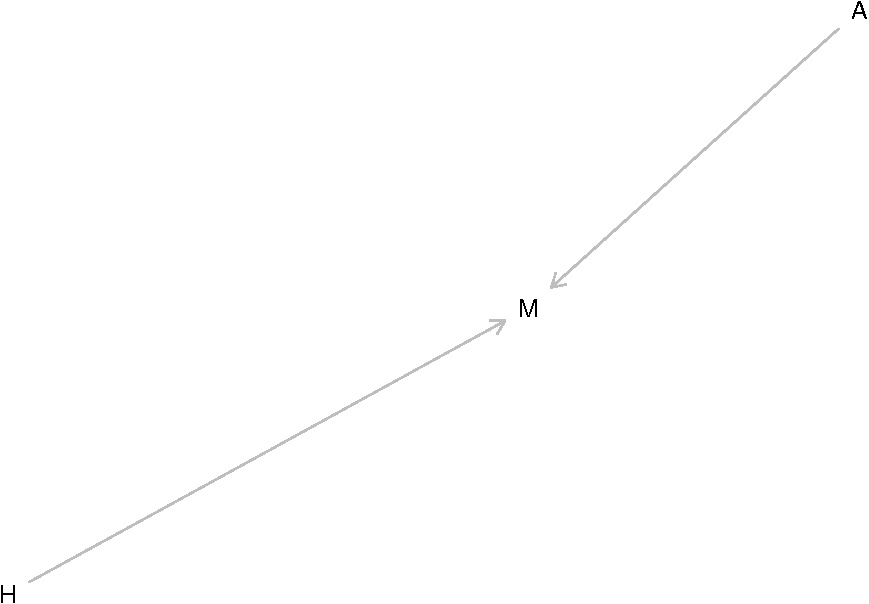
\includegraphics{rethinkingINLA_HW4_files/figure-latex/hw4.2 dag-1.pdf}

Happiness (H) and age (A) both cause marriage (M). Marriage is therefore
a collider. Even though there is no causal association between happiness
and age, if we condition on marriage--- which means here, if we include
it as a predictor in a regression---then it will induce a statistical
association between age and happiness. And this can mislead us to think
that happiness changes with age, when in fact it is constant.

Run models m6.9 and m6.10 again. Compare these two models using WAIC (or
LOO, they will produce identical results). Which model is expected to
make better predictions? Which model provides the correct causal
inference about the influence of age on happiness? Can you explain why
the answers to these two questions disagree?

SOL: So let's consider a multiple regression model aimed at inferring
the influence of age on happiness, while controlling for marriage
status. This is just a plain multiple regression, like the others in
this and the previous chapter.

The linear model is this: \(\mu_i= \alpha mid[i] + \beta AA_i\) where
mid{[}i{]} is an index for the marriage status of individual i, with 1
meaning single and 2 meaning married. It's easier to make priors, when
we use multiple intercepts, one for each category, than when we use
indicator variables.

Now we should do our duty and think about the priors.

\begin{itemize}
\item
  Let's consider the slope \(\beta A\) first, because how we scale the
  predictor A will determine the meaning of the intercept. We'll focus
  only on the adult sample, those 18 or over. Imagine a very strong
  relationship between age and happiness, such that happiness is at its
  maximum at age 18 and its minimum at age 65. It'll be easier if we
  rescale age so that the range from 18 to 65 is one unit. Now this new
  variable A ranges from 0 to 1, where 0 is age 18 and 1 is age 65.
\item
  Happiness is on an arbitrary scale, in these data, from −2 to +2. So
  our imaginary strongest relationship, taking happiness from maximum to
  minimum, has a slope with rise over run of (2 − (−2))/1 = 4. Remember
  that 95\% of the mass of a normal distribution is contained within 2
  standard deviations. So if we set the standard deviation of the prior
  to half of 4, we are saying that we expect 95\% of plausible slopes to
  be less than maximally strong. That isn't a very strong prior, but
  again, it at least helps bound inference to realistic ranges.
\item
  Now for the intercepts. Each α is the value of \(\mu_i\) when Ai = 0.
  In this case, that means at age 18. So we need to allow \(\alpha\) to
  cover the full range of happiness scores. Normal(0, 1) will put 95\%
  of the mass in the −2 to +2 interval.
\item
  We need to construct the marriage status index variable, as well.
\end{itemize}

Finally, let's approximate the posterior.

\begin{Shaded}
\begin{Highlighting}[]
\NormalTok{d <-}\StringTok{ }\KeywordTok{sim_happiness}\NormalTok{( }\DataTypeTok{seed=}\DecValTok{1977}\NormalTok{ , }\DataTypeTok{N_years=}\DecValTok{1000}\NormalTok{ )}
\NormalTok{d2 <-}\StringTok{ }\NormalTok{d[ d}\OperatorTok{$}\NormalTok{age}\OperatorTok{>}\DecValTok{17}\NormalTok{ , ] }\CommentTok{# only adults}
\NormalTok{d2}\OperatorTok{$}\NormalTok{A <-}\StringTok{ }\NormalTok{( d2}\OperatorTok{$}\NormalTok{age }\OperatorTok{-}\StringTok{ }\DecValTok{18}\NormalTok{ ) }\OperatorTok{/}\StringTok{ }\NormalTok{( }\DecValTok{65} \OperatorTok{-}\StringTok{ }\DecValTok{18}\NormalTok{ )}
\NormalTok{d2}\OperatorTok{$}\NormalTok{mid <-}\StringTok{ }\NormalTok{d2}\OperatorTok{$}\NormalTok{married }\OperatorTok{+}\StringTok{ }\DecValTok{1}
\end{Highlighting}
\end{Shaded}

Model m6.9 contains both marriage status and age. Model m6.10 contains
only age. Model m6.9 produces a confounded inference about the
relationship between age and happiness, due to opening a collider path.

\hypertarget{rethinking}{%
\subsubsection{rethinking}\label{rethinking}}

\begin{Shaded}
\begin{Highlighting}[]
\CommentTok{#contains both marriage status and age}

\NormalTok{m6}\FloatTok{.9}\NormalTok{ <-}\StringTok{ }\KeywordTok{quap}\NormalTok{(}
    \KeywordTok{alist}\NormalTok{(}
\NormalTok{        happiness }\OperatorTok{~}\StringTok{ }\KeywordTok{dnorm}\NormalTok{( mu , sigma ),}
\NormalTok{        mu <-}\StringTok{ }\NormalTok{a[mid] }\OperatorTok{+}\StringTok{ }\NormalTok{bA}\OperatorTok{*}\NormalTok{A,}
\NormalTok{        a[mid] }\OperatorTok{~}\StringTok{ }\KeywordTok{dnorm}\NormalTok{( }\DecValTok{0}\NormalTok{ , }\DecValTok{1}\NormalTok{ ),}
\NormalTok{        bA }\OperatorTok{~}\StringTok{ }\KeywordTok{dnorm}\NormalTok{( }\DecValTok{0}\NormalTok{ , }\DecValTok{2}\NormalTok{ ),}
\NormalTok{        sigma }\OperatorTok{~}\StringTok{ }\KeywordTok{dexp}\NormalTok{(}\DecValTok{1}\NormalTok{)}
\NormalTok{    ) , }\DataTypeTok{data=}\NormalTok{d2 )}
\KeywordTok{precis}\NormalTok{(m6}\FloatTok{.9}\NormalTok{,}\DataTypeTok{depth=}\DecValTok{2}\NormalTok{)}
\end{Highlighting}
\end{Shaded}

\begin{verbatim}
##             mean         sd       5.5%      94.5%
## a[1]  -0.2350877 0.06348986 -0.3365568 -0.1336186
## a[2]   1.2585517 0.08495989  1.1227694  1.3943340
## bA    -0.7490274 0.11320112 -0.9299447 -0.5681102
## sigma  0.9897080 0.02255800  0.9536559  1.0257600
\end{verbatim}

\hypertarget{inla}{%
\subsubsection{INLA}\label{inla}}

In order to code a separate intercept for being married/not, we need to
reformat the data so that there are separate variables for each
intercept, with 1s for a given value of the variable we are basing the
intercept on ( in this case marriage) and NAs for all other values.

\begin{Shaded}
\begin{Highlighting}[]
\NormalTok{d3 <-}\StringTok{ }\NormalTok{d2 }\OperatorTok\StringTok{ }
\StringTok{  }\KeywordTok{mutate}\NormalTok{(}\DataTypeTok{i_notmarried=} \KeywordTok{na_if}\NormalTok{(}\KeywordTok{if_else}\NormalTok{(married}\OperatorTok{==}\DecValTok{0}\NormalTok{, }\DecValTok{1}\NormalTok{, }\DecValTok{0}\NormalTok{), }\DecValTok{0}\NormalTok{), }
         \DataTypeTok{i_married=} \KeywordTok{na_if}\NormalTok{(married, }\DecValTok{0}\NormalTok{)) }

\NormalTok{m6.}\FloatTok{9.}\NormalTok{inla.prior <-}\StringTok{ }\KeywordTok{inla}\NormalTok{(happiness}\OperatorTok{~}\StringTok{ }\DecValTok{-1} \OperatorTok{+}\NormalTok{i_notmarried}\OperatorTok{+}\NormalTok{i_married }\OperatorTok{+}\StringTok{ }\NormalTok{A , }\DataTypeTok{data=}\NormalTok{ d3, }
                        \DataTypeTok{control.fixed =} \KeywordTok{list}\NormalTok{(}
        \DataTypeTok{mean=} \KeywordTok{list}\NormalTok{(}\DecValTok{0}\NormalTok{), }
        \DataTypeTok{prec=} \KeywordTok{list}\NormalTok{(}\DataTypeTok{i_notmarried=}\DecValTok{2}\NormalTok{, }\DataTypeTok{i_married=} \DecValTok{1}\NormalTok{, }\DataTypeTok{A=}\DecValTok{2}\NormalTok{)),}
        \DataTypeTok{control.compute =} \KeywordTok{list}\NormalTok{(}\DataTypeTok{dic=}\OtherTok{TRUE}\NormalTok{, }\DataTypeTok{waic=} \OtherTok{TRUE}\NormalTok{)}
\NormalTok{)}

\KeywordTok{summary}\NormalTok{(m6.}\FloatTok{9.}\NormalTok{inla.prior )}
\end{Highlighting}
\end{Shaded}

\begin{verbatim}
## 
## Call:
##    c("inla(formula = happiness ~ -1 + i_notmarried + i_married + A, ", " data = d3, 
##    control.compute = list(dic = TRUE, waic = TRUE), ", " control.fixed = list(mean 
##    = list(0), prec = list(i_notmarried = 2, ", " i_married = 1, A = 2)))") 
## Time used:
##     Pre = 1.14, Running = 0.462, Post = 0.231, Total = 1.83 
## Fixed effects:
##                mean    sd 0.025quant 0.5quant 0.975quant   mode kld
## i_notmarried -0.240 0.063     -0.364   -0.240     -0.116 -0.240   0
## i_married     1.251 0.084      1.085    1.251      1.416  1.251   0
## A            -0.736 0.112     -0.956   -0.736     -0.516 -0.736   0
## 
## Model hyperparameters:
##                                         mean    sd 0.025quant 0.5quant 0.975quant mode
## Precision for the Gaussian observations 1.02 0.046       0.93     1.02       1.11 1.02
## 
## Expected number of effective parameters(stdev): 2.97(0.002)
## Number of equivalent replicates : 323.69 
## 
## Deviance Information Criterion (DIC) ...............: 2714.19
## Deviance Information Criterion (DIC, saturated) ....: 967.05
## Effective number of parameters .....................: 4.00
## 
## Watanabe-Akaike information criterion (WAIC) ...: 2713.83
## Effective number of parameters .................: 3.62
## 
## Marginal log-Likelihood:  -1374.21 
## Posterior marginals for the linear predictor and
##  the fitted values are computed
\end{verbatim}

\hypertarget{rethinking-1}{%
\subsubsection{rethinking}\label{rethinking-1}}

\begin{Shaded}
\begin{Highlighting}[]
\CommentTok{#this model to a model that omits marriage status.}
\NormalTok{m6}\FloatTok{.10}\NormalTok{ <-}\StringTok{ }\KeywordTok{quap}\NormalTok{(}
    \KeywordTok{alist}\NormalTok{(}
\NormalTok{        happiness }\OperatorTok{~}\StringTok{ }\KeywordTok{dnorm}\NormalTok{( mu , sigma ),}
\NormalTok{        mu <-}\StringTok{ }\NormalTok{a }\OperatorTok{+}\StringTok{ }\NormalTok{bA}\OperatorTok{*}\NormalTok{A,}
\NormalTok{        a }\OperatorTok{~}\StringTok{ }\KeywordTok{dnorm}\NormalTok{( }\DecValTok{0}\NormalTok{ , }\DecValTok{1}\NormalTok{ ),}
\NormalTok{        bA }\OperatorTok{~}\StringTok{ }\KeywordTok{dnorm}\NormalTok{( }\DecValTok{0}\NormalTok{ , }\DecValTok{2}\NormalTok{ ),}
\NormalTok{        sigma }\OperatorTok{~}\StringTok{ }\KeywordTok{dexp}\NormalTok{(}\DecValTok{1}\NormalTok{)}
\NormalTok{    ) , }\DataTypeTok{data=}\NormalTok{d2 )}
\KeywordTok{precis}\NormalTok{(m6}\FloatTok{.10}\NormalTok{)}
\end{Highlighting}
\end{Shaded}

\begin{verbatim}
##                mean         sd       5.5%     94.5%
## a     -1.469528e-06 0.07675016 -0.1226630 0.1226601
## bA     2.378318e-06 0.13225977 -0.2113743 0.2113790
## sigma  1.213188e+00 0.02766081  1.1689804 1.2573950
\end{verbatim}

\hypertarget{inla-1}{%
\subsubsection{INLA}\label{inla-1}}

\begin{Shaded}
\begin{Highlighting}[]
\NormalTok{m6.}\FloatTok{10.}\NormalTok{inla.prior <-}\StringTok{ }\KeywordTok{inla}\NormalTok{(happiness}\OperatorTok{~}\StringTok{ }\NormalTok{A , }\DataTypeTok{data=}\NormalTok{ d3, }
                        \DataTypeTok{control.fixed =} \KeywordTok{list}\NormalTok{(}
        \DataTypeTok{mean=} \KeywordTok{list}\NormalTok{(}\DecValTok{0}\NormalTok{), }
        \DataTypeTok{prec=} \KeywordTok{list}\NormalTok{(}\DecValTok{2}\NormalTok{),}
        \DataTypeTok{mean.intercept=} \DecValTok{0}\NormalTok{, }
        \DataTypeTok{prec.intercept=} \DecValTok{1}\NormalTok{),}
        \DataTypeTok{control.compute =} \KeywordTok{list}\NormalTok{(}\DataTypeTok{dic=}\OtherTok{TRUE}\NormalTok{, }\DataTypeTok{waic=} \OtherTok{TRUE}\NormalTok{)}
\NormalTok{)}

\KeywordTok{summary}\NormalTok{(m6.}\FloatTok{10.}\NormalTok{inla.prior )}
\end{Highlighting}
\end{Shaded}

\begin{verbatim}
## 
## Call:
##    c("inla(formula = happiness ~ A, data = d3, control.compute = list(dic = TRUE, 
##    ", " waic = TRUE), control.fixed = list(mean = list(0), prec = list(2), ", " 
##    mean.intercept = 0, prec.intercept = 1))") 
## Time used:
##     Pre = 1.12, Running = 0.456, Post = 0.219, Total = 1.8 
## Fixed effects:
##             mean    sd 0.025quant 0.5quant 0.975quant mode kld
## (Intercept)    0 0.077     -0.151        0      0.151    0   0
## A              0 0.133     -0.261        0      0.260    0   0
## 
## Model hyperparameters:
##                                          mean    sd 0.025quant 0.5quant 0.975quant  mode
## Precision for the Gaussian observations 0.679 0.031       0.62    0.678       0.74 0.677
## 
## Expected number of effective parameters(stdev): 2.00(0.00)
## Number of equivalent replicates : 480.47 
## 
## Deviance Information Criterion (DIC) ...............: 3102.68
## Deviance Information Criterion (DIC, saturated) ....: 966.07
## Effective number of parameters .....................: 3.04
## 
## Watanabe-Akaike information criterion (WAIC) ...: 3102.06
## Effective number of parameters .................: 2.41
## 
## Marginal log-Likelihood:  -1569.48 
## Posterior marginals for the linear predictor and
##  the fitted values are computed
\end{verbatim}

\hypertarget{to-compare-these-models-using-waic}{%
\subsubsection{To compare these models using
WAIC:}\label{to-compare-these-models-using-waic}}

\begin{Shaded}
\begin{Highlighting}[]
\CommentTok{#rethinking}
 \KeywordTok{compare}\NormalTok{( m6}\FloatTok{.9}\NormalTok{ , m6}\FloatTok{.10}\NormalTok{ )}
\end{Highlighting}
\end{Shaded}

\begin{verbatim}
##           WAIC       SE    dWAIC      dSE    pWAIC       weight
## m6.9  2713.964 37.55324   0.0000       NA 3.732484 1.000000e+00
## m6.10 3101.906 27.74820 387.9425 35.41158 2.337316 5.745894e-85
\end{verbatim}

\begin{Shaded}
\begin{Highlighting}[]
\CommentTok{# INLA }
\NormalTok{m6.}\FloatTok{9.}\NormalTok{inla.prior}\OperatorTok{$}\NormalTok{waic}\OperatorTok{$}\NormalTok{waic}
\end{Highlighting}
\end{Shaded}

\begin{verbatim}
## [1] 2713.829
\end{verbatim}

\begin{Shaded}
\begin{Highlighting}[]
\NormalTok{m6.}\FloatTok{10.}\NormalTok{inla.prior}\OperatorTok{$}\NormalTok{waic}\OperatorTok{$}\NormalTok{waic}
\end{Highlighting}
\end{Shaded}

\begin{verbatim}
## [1] 3102.064
\end{verbatim}

The model that produces the invalid inference, m6.9, is expected to
predict much better. And it would. This is because the collider path
does convey actual association. We simply end up mistaken about the
causal inference. We should not use WAIC (or LOO) to choose among
models, unless we have some clear sense of the causal model. These
criteria will happily favor confounded models.

\hypertarget{section-2}{%
\subsection{3.}\label{section-2}}

Reconsider the urban fox analysis from last week's homework. Use WAIC or
LOO based model comparison on five different models, each using weight
as the outcome, and containing these sets of predictor variables: (1)
avgfood + groupsize + area (2) avgfood + groupsize (3) groupsize + area
(4) avgfood (5) area

Can you explain the relative differences in WAIC scores, using the fox
DAG from last week's homework? Be sure to pay attention to the standard
error of the score differences (dSE).

\begin{verbatim}
## Plot coordinates for graph not supplied! Generating coordinates, see ?coordinates for how to set your own.
\end{verbatim}

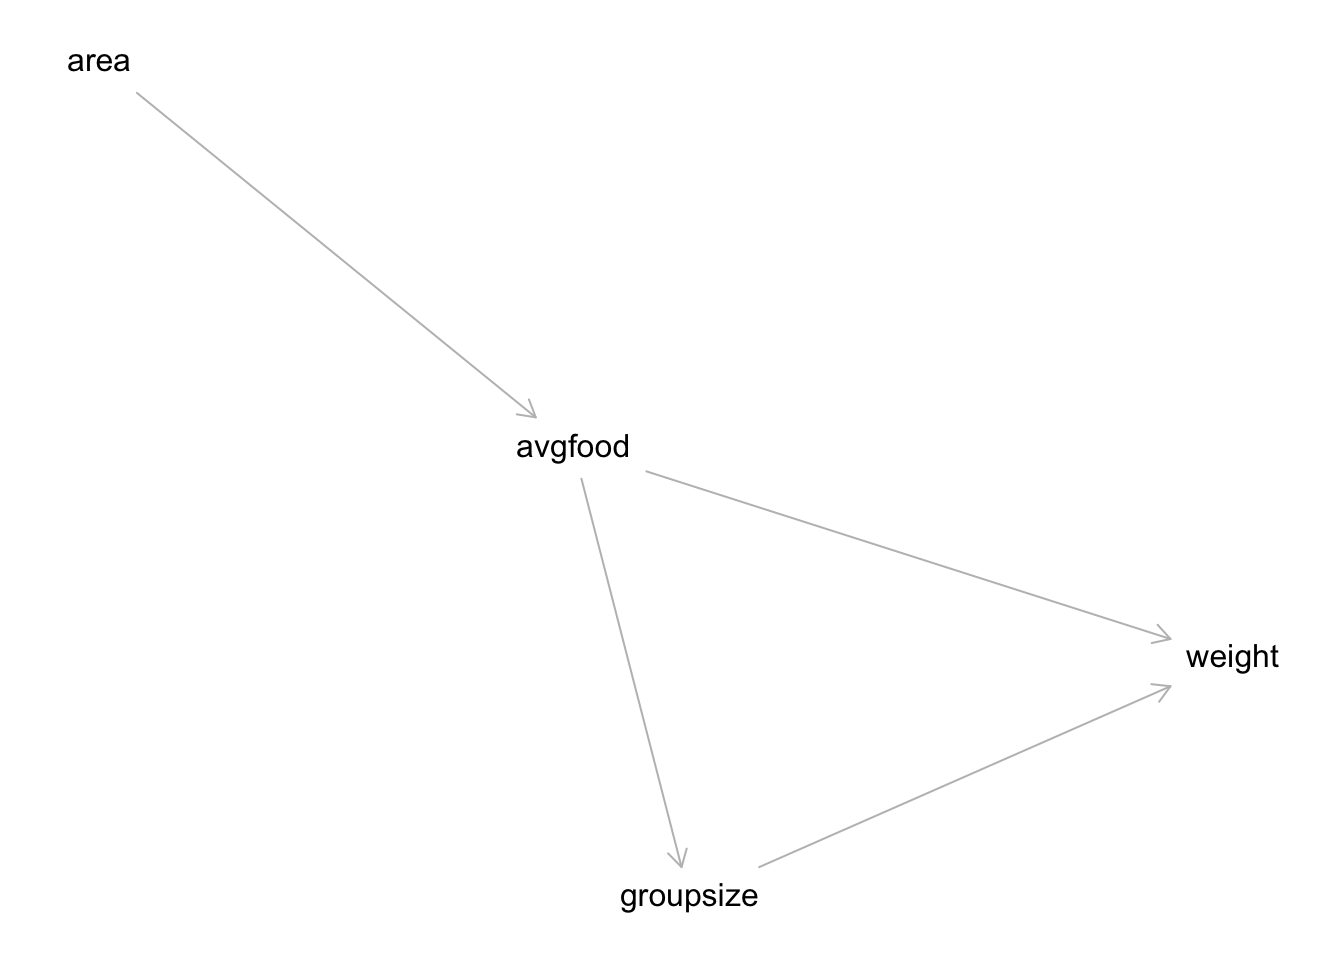
\includegraphics{rethinkingINLA_HW4_files/figure-latex/hw3 dag-1.pdf}

\begin{Shaded}
\begin{Highlighting}[]
\KeywordTok{library}\NormalTok{(rethinking)}
\KeywordTok{data}\NormalTok{(foxes)}
\NormalTok{d <-}\StringTok{ }\NormalTok{foxes}
\NormalTok{d}\OperatorTok{$}\NormalTok{W <-}\StringTok{ }\KeywordTok{standardize}\NormalTok{(d}\OperatorTok{$}\NormalTok{weight)}
\NormalTok{d}\OperatorTok{$}\NormalTok{A <-}\StringTok{ }\KeywordTok{standardize}\NormalTok{(d}\OperatorTok{$}\NormalTok{area)}
\NormalTok{d}\OperatorTok{$}\NormalTok{F <-}\StringTok{ }\KeywordTok{standardize}\NormalTok{(d}\OperatorTok{$}\NormalTok{avgfood)}
\NormalTok{d}\OperatorTok{$}\NormalTok{G <-}\StringTok{ }\KeywordTok{standardize}\NormalTok{(d}\OperatorTok{$}\NormalTok{groupsize)}
\end{Highlighting}
\end{Shaded}

\hypertarget{rethinking-2}{%
\subsubsection{rethinking}\label{rethinking-2}}

\begin{Shaded}
\begin{Highlighting}[]
\NormalTok{m1 <-}\StringTok{ }\KeywordTok{quap}\NormalTok{(}
    \KeywordTok{alist}\NormalTok{(}
\NormalTok{        W }\OperatorTok{~}\StringTok{ }\KeywordTok{dnorm}\NormalTok{( mu , sigma ),}
\NormalTok{        mu <-}\StringTok{ }\NormalTok{a }\OperatorTok{+}\StringTok{ }\NormalTok{bF}\OperatorTok{*}\NormalTok{F }\OperatorTok{+}\StringTok{ }\NormalTok{bG}\OperatorTok{*}\NormalTok{G }\OperatorTok{+}\StringTok{ }\NormalTok{bA}\OperatorTok{*}\NormalTok{A,}
\NormalTok{        a }\OperatorTok{~}\StringTok{ }\KeywordTok{dnorm}\NormalTok{(}\DecValTok{0}\NormalTok{,}\FloatTok{0.2}\NormalTok{),}
        \KeywordTok{c}\NormalTok{(bF,bG,bA) }\OperatorTok{~}\StringTok{ }\KeywordTok{dnorm}\NormalTok{(}\DecValTok{0}\NormalTok{,}\FloatTok{0.5}\NormalTok{),}
\NormalTok{        sigma }\OperatorTok{~}\StringTok{ }\KeywordTok{dexp}\NormalTok{(}\DecValTok{1}\NormalTok{)}
\NormalTok{    ), }\DataTypeTok{data=}\NormalTok{d )}
\NormalTok{m2 <-}\StringTok{ }\KeywordTok{quap}\NormalTok{(}
    \KeywordTok{alist}\NormalTok{(}
\NormalTok{        W }\OperatorTok{~}\StringTok{ }\KeywordTok{dnorm}\NormalTok{( mu , sigma ),}
\NormalTok{        mu <-}\StringTok{ }\NormalTok{a }\OperatorTok{+}\StringTok{ }\NormalTok{bF}\OperatorTok{*}\NormalTok{F }\OperatorTok{+}\StringTok{ }\NormalTok{bG}\OperatorTok{*}\NormalTok{G,}
\NormalTok{        a }\OperatorTok{~}\StringTok{ }\KeywordTok{dnorm}\NormalTok{(}\DecValTok{0}\NormalTok{,}\FloatTok{0.2}\NormalTok{),}
        \KeywordTok{c}\NormalTok{(bF,bG) }\OperatorTok{~}\StringTok{ }\KeywordTok{dnorm}\NormalTok{(}\DecValTok{0}\NormalTok{,}\FloatTok{0.5}\NormalTok{),}
\NormalTok{        sigma }\OperatorTok{~}\StringTok{ }\KeywordTok{dexp}\NormalTok{(}\DecValTok{1}\NormalTok{)}
\NormalTok{    ), }\DataTypeTok{data=}\NormalTok{d )}
\NormalTok{m3 <-}\StringTok{ }\KeywordTok{quap}\NormalTok{(}
    \KeywordTok{alist}\NormalTok{(}
\NormalTok{        W }\OperatorTok{~}\StringTok{ }\KeywordTok{dnorm}\NormalTok{( mu , sigma ),}
\NormalTok{        mu <-}\StringTok{ }\NormalTok{a }\OperatorTok{+}\StringTok{ }\NormalTok{bG}\OperatorTok{*}\NormalTok{G }\OperatorTok{+}\StringTok{ }\NormalTok{bA}\OperatorTok{*}\NormalTok{A,}
\NormalTok{        a }\OperatorTok{~}\StringTok{ }\KeywordTok{dnorm}\NormalTok{(}\DecValTok{0}\NormalTok{,}\FloatTok{0.2}\NormalTok{),}
        \KeywordTok{c}\NormalTok{(bG,bA) }\OperatorTok{~}\StringTok{ }\KeywordTok{dnorm}\NormalTok{(}\DecValTok{0}\NormalTok{,}\FloatTok{0.5}\NormalTok{),}
\NormalTok{        sigma }\OperatorTok{~}\StringTok{ }\KeywordTok{dexp}\NormalTok{(}\DecValTok{1}\NormalTok{)}
\NormalTok{    ), }\DataTypeTok{data=}\NormalTok{d )}
\NormalTok{m4 <-}\StringTok{ }\KeywordTok{quap}\NormalTok{(}
    \KeywordTok{alist}\NormalTok{(}
\NormalTok{        W }\OperatorTok{~}\StringTok{ }\KeywordTok{dnorm}\NormalTok{( mu , sigma ),}
\NormalTok{        mu <-}\StringTok{ }\NormalTok{a }\OperatorTok{+}\StringTok{ }\NormalTok{bF}\OperatorTok{*}\NormalTok{F,}
\NormalTok{        a }\OperatorTok{~}\StringTok{ }\KeywordTok{dnorm}\NormalTok{(}\DecValTok{0}\NormalTok{,}\FloatTok{0.2}\NormalTok{),}
\NormalTok{        bF }\OperatorTok{~}\StringTok{ }\KeywordTok{dnorm}\NormalTok{(}\DecValTok{0}\NormalTok{,}\FloatTok{0.5}\NormalTok{),}
\NormalTok{        sigma }\OperatorTok{~}\StringTok{ }\KeywordTok{dexp}\NormalTok{(}\DecValTok{1}\NormalTok{)}
\NormalTok{    ), }\DataTypeTok{data=}\NormalTok{d )}
\NormalTok{m5 <-}\StringTok{ }\KeywordTok{quap}\NormalTok{(}
    \KeywordTok{alist}\NormalTok{(}
\NormalTok{        W }\OperatorTok{~}\StringTok{ }\KeywordTok{dnorm}\NormalTok{( mu , sigma ),}
\NormalTok{        mu <-}\StringTok{ }\NormalTok{a }\OperatorTok{+}\StringTok{ }\NormalTok{bA}\OperatorTok{*}\NormalTok{A,}
\NormalTok{        a }\OperatorTok{~}\StringTok{ }\KeywordTok{dnorm}\NormalTok{(}\DecValTok{0}\NormalTok{,}\FloatTok{0.2}\NormalTok{),}
\NormalTok{        bA }\OperatorTok{~}\StringTok{ }\KeywordTok{dnorm}\NormalTok{(}\DecValTok{0}\NormalTok{,}\FloatTok{0.5}\NormalTok{),}
\NormalTok{        sigma }\OperatorTok{~}\StringTok{ }\KeywordTok{dexp}\NormalTok{(}\DecValTok{1}\NormalTok{)}
\NormalTok{), }\DataTypeTok{data=}\NormalTok{d )}


 \KeywordTok{compare}\NormalTok{( m1 , m2 , m3 , m4 , m5 )}
\end{Highlighting}
\end{Shaded}

\begin{verbatim}
##        WAIC       SE     dWAIC      dSE    pWAIC      weight
## m1 322.8570 16.27702  0.000000       NA 4.643026 0.464863619
## m3 323.8852 15.67222  1.028262 2.911577 3.711944 0.277997758
## m2 324.0754 16.12771  1.218433 3.584892 3.818873 0.252782029
## m4 333.4369 13.78791 10.579891 7.194478 2.423844 0.002343859
## m5 333.7415 13.79359 10.884499 7.243278 2.659040 0.002012735
\end{verbatim}

\hypertarget{inla-2}{%
\subsubsection{INLA}\label{inla-2}}

\begin{Shaded}
\begin{Highlighting}[]
\NormalTok{m1.i <-}\StringTok{ }\KeywordTok{inla}\NormalTok{(W}\OperatorTok{~}\NormalTok{F}\OperatorTok{+}\NormalTok{G}\OperatorTok{+}\NormalTok{A, }\DataTypeTok{data=}\NormalTok{ d, }\DataTypeTok{control.fixed =} \KeywordTok{list}\NormalTok{(}
        \DataTypeTok{mean=} \KeywordTok{list}\NormalTok{(}\DecValTok{0}\NormalTok{), }
        \DataTypeTok{prec=} \KeywordTok{list}\NormalTok{(}\DataTypeTok{F=}\FloatTok{0.5}\NormalTok{, }\DataTypeTok{G=}\FloatTok{0.5}\NormalTok{, }\DataTypeTok{A=} \FloatTok{0.5}\NormalTok{), }
        \DataTypeTok{mean.intercept=} \DecValTok{0}\NormalTok{, }
        \DataTypeTok{prec.intercept=} \FloatTok{0.2}
\NormalTok{), }
\DataTypeTok{control.compute =} \KeywordTok{list}\NormalTok{(}\DataTypeTok{waic=} \OtherTok{TRUE}\NormalTok{))}
\CommentTok{#summary(m1.i)}

\NormalTok{m2.i <-}\StringTok{ }\KeywordTok{inla}\NormalTok{(W}\OperatorTok{~}\NormalTok{F}\OperatorTok{+}\NormalTok{G, }\DataTypeTok{data=}\NormalTok{ d, }\DataTypeTok{control.fixed =} \KeywordTok{list}\NormalTok{(}
        \DataTypeTok{mean=} \KeywordTok{list}\NormalTok{(}\DecValTok{0}\NormalTok{), }
        \DataTypeTok{prec=} \KeywordTok{list}\NormalTok{(}\DataTypeTok{F=}\FloatTok{0.5}\NormalTok{, }\DataTypeTok{G=}\FloatTok{0.5}\NormalTok{), }
        \DataTypeTok{mean.intercept=} \DecValTok{0}\NormalTok{, }
        \DataTypeTok{prec.intercept=} \FloatTok{0.2}
\NormalTok{), }
\DataTypeTok{control.compute =} \KeywordTok{list}\NormalTok{(}\DataTypeTok{waic=} \OtherTok{TRUE}\NormalTok{))}
\CommentTok{#summary(m2.i)}

\NormalTok{m3.i <-}\StringTok{ }\KeywordTok{inla}\NormalTok{(W}\OperatorTok{~}\NormalTok{A}\OperatorTok{+}\NormalTok{G, }\DataTypeTok{data=}\NormalTok{ d, }\DataTypeTok{control.fixed =} \KeywordTok{list}\NormalTok{(}
        \DataTypeTok{mean=} \KeywordTok{list}\NormalTok{(}\DecValTok{0}\NormalTok{), }
        \DataTypeTok{prec=} \KeywordTok{list}\NormalTok{(}\DataTypeTok{A=}\FloatTok{0.5}\NormalTok{, }\DataTypeTok{G=}\FloatTok{0.5}\NormalTok{), }
        \DataTypeTok{mean.intercept=} \DecValTok{0}\NormalTok{, }
        \DataTypeTok{prec.intercept=} \FloatTok{0.2}
\NormalTok{), }
\DataTypeTok{control.compute =} \KeywordTok{list}\NormalTok{(}\DataTypeTok{waic=} \OtherTok{TRUE}\NormalTok{))}
\CommentTok{#summary(m3.i)}

\NormalTok{m4.i <-}\StringTok{ }\KeywordTok{inla}\NormalTok{(W}\OperatorTok{~}\NormalTok{F, }\DataTypeTok{data=}\NormalTok{ d, }\DataTypeTok{control.fixed =} \KeywordTok{list}\NormalTok{(}
        \DataTypeTok{mean=} \KeywordTok{list}\NormalTok{(}\DecValTok{0}\NormalTok{), }
        \DataTypeTok{prec=} \KeywordTok{list}\NormalTok{(}\FloatTok{0.5}\NormalTok{), }
        \DataTypeTok{mean.intercept=} \DecValTok{0}\NormalTok{, }
        \DataTypeTok{prec.intercept=} \FloatTok{0.2}
\NormalTok{), }
\DataTypeTok{control.compute =} \KeywordTok{list}\NormalTok{(}\DataTypeTok{waic=} \OtherTok{TRUE}\NormalTok{))}
\CommentTok{#summary(m4.i)}

\NormalTok{m5.i <-}\StringTok{ }\KeywordTok{inla}\NormalTok{(W}\OperatorTok{~}\NormalTok{A, }\DataTypeTok{data=}\NormalTok{ d, }\DataTypeTok{control.fixed =} \KeywordTok{list}\NormalTok{(}
        \DataTypeTok{mean=} \KeywordTok{list}\NormalTok{(}\DecValTok{0}\NormalTok{), }
        \DataTypeTok{prec=} \KeywordTok{list}\NormalTok{(}\FloatTok{0.5}\NormalTok{), }
        \DataTypeTok{mean.intercept=} \DecValTok{0}\NormalTok{, }
        \DataTypeTok{prec.intercept=} \FloatTok{0.2}
\NormalTok{), }
\DataTypeTok{control.compute =} \KeywordTok{list}\NormalTok{(}\DataTypeTok{waic=} \OtherTok{TRUE}\NormalTok{))}
\CommentTok{#summary(m5.i)}

\NormalTok{m1.i}\OperatorTok{$}\NormalTok{waic}\OperatorTok{$}\NormalTok{waic}
\end{Highlighting}
\end{Shaded}

\begin{verbatim}
## [1] 323.5388
\end{verbatim}

\begin{Shaded}
\begin{Highlighting}[]
\NormalTok{m2.i}\OperatorTok{$}\NormalTok{waic}\OperatorTok{$}\NormalTok{waic}
\end{Highlighting}
\end{Shaded}

\begin{verbatim}
## [1] 323.8215
\end{verbatim}

\begin{Shaded}
\begin{Highlighting}[]
\NormalTok{m3.i}\OperatorTok{$}\NormalTok{waic}\OperatorTok{$}\NormalTok{waic}
\end{Highlighting}
\end{Shaded}

\begin{verbatim}
## [1] 324.1259
\end{verbatim}

\begin{Shaded}
\begin{Highlighting}[]
\NormalTok{m4.i}\OperatorTok{$}\NormalTok{waic}\OperatorTok{$}\NormalTok{waic}
\end{Highlighting}
\end{Shaded}

\begin{verbatim}
## [1] 333.8307
\end{verbatim}

\begin{Shaded}
\begin{Highlighting}[]
\NormalTok{m5.i}\OperatorTok{$}\NormalTok{waic}\OperatorTok{$}\NormalTok{waic}
\end{Highlighting}
\end{Shaded}

\begin{verbatim}
## [1] 334.0923
\end{verbatim}

Notice that the top three models are m1, m3, and m2. They have very
similar WAIC values. The differences are small and smaller in all cases
than the standard error of the difference. WAIC sees these models are
tied. This makes sense, given the DAG, because as long as a model has
groupsize in it, we can include either avgfood or area or both and get
the same inferences. Another way to think of this is that the influence
of good, adjusting for group size, is (according to the DAG) the same as
the influence of area, adjusting for group size, because the influence
of area is routed entirely through food and group size. There are no
backdoor paths. What about the other two models, m4 and m5? These models
are tied with one another, and both omit group size. Again, the
influence of area passes entirely through food. So including only food
or only area should produce the same inference---the total causal
influence of area (or food) is just about zero. That's indeed what the
posterior distributions suggest:

\begin{Shaded}
\begin{Highlighting}[]
\KeywordTok{coeftab}\NormalTok{(m4,m5)}
\end{Highlighting}
\end{Shaded}

\begin{verbatim}
##       m4      m5     
## a           0       0
## bF      -0.02      NA
## sigma    0.99    0.99
## bA         NA    0.02
## nobs      116     116
\end{verbatim}

\end{document}
